\documentclass[conference]{IEEEtran}
\IEEEoverridecommandlockouts
% The preceding line is only needed to identify funding in the first footnote. If that is unneeded, please comment it out.
\usepackage[nocompress]{cite}
\renewcommand{\citepunct}{][}
\usepackage{amsmath,amssymb,amsfonts}
\usepackage{algorithmic}
\usepackage{graphicx}
\usepackage{textcomp}
\usepackage{xcolor}
\usepackage{booktabs}
\usepackage{float}
\def\BibTeX{{\rm B\kern-.05em{\sc i\kern-.025em b}\kern-.08em
    T\kern-.1667em\lower.7ex\hbox{E}\kern-.125emX}}
\raggedbottom
\begin{document}

\title{TempoRF-DETR: Video-Based Coronary Stenosis Detection with Image-to-Video Distillation\\
\thanks{This thesis was prepared in partial fulfilment of the requirements for the Degree of Bachelor of Science in Data Science and Artificial Intelligence, Maastricht University. Supervisor(s): Yusuf Can Semeri, Mark Punt}
}

\author{\IEEEauthorblockN{Dmitrii Sakharov}
\IEEEauthorblockA{\textit{Department of Advanced Computing Sciences} \\
\textit{Faculty of Science and Engineering}\\
\textit{Maastricht University}\\
Maastricht, The Netherlands}
}

\maketitle

\begin{abstract}
Video-based coronary stenosis detection in X-ray angiography promises higher accuracy than single-frame detection by aggregating cardiac and respiratory motion across consecutive frames, but is constrained by labeled data: per-frame box annotations are expensive, and most publicly available stenosis resources are released as single-frame images rather than video sequences. We propose TempoRF-DETR, a video extension of RF-DETR that exchanges context across all frames of a clip in a single forward pass via an Early Temporal Fusion (ETF) module. To compensate for the smaller video dataset, we introduce an image-to-video knowledge distillation scheme: a frozen 2D RF-DETR teacher pre-trained on the union of a single-frame dataset and decoded video frames supervises the video student model per frame via query-aligned distillation (KD-DETR), general-query sampling, and cross-resolution relational contrastive distillation (CRRCD). TempoRF-DETR reaches micro-pooled AP at IoU 0.30 of $0.581$ on the in-distribution test set and transfers without retraining to $0.416$ on the out-of-distribution CADICA dataset, $+0.246$ AP$_{30}$ above the strongest reimplemented video baseline and $+0.063$ above the strongest parameter-efficient alternative.
\end{abstract}

\begin{IEEEkeywords}
coronary stenosis detection, X-ray angiography, video object detection, DETR, knowledge distillation, image-to-video transfer, parameter-efficient tuning
\end{IEEEkeywords}

\section{Introduction}

Coronary artery disease (CAD) is one of the leading causes of mortality worldwide, driven by the build-up of atherosclerotic plaque that narrows (stenosis) the coronary arteries~\cite{popov2022reviewmodernapproachescoronary}. X-ray coronary angiography (XCA) is the clinical gold standard for assessing stenosis severity, but its interpretation exhibits substantial inter- and intra-observer variability~\cite{zir1976interobserver, cardiovascular}, which directly affects treatment decisions. Automated stenosis detection in XCA is therefore of considerable clinical value, yet it remains challenging: vessels overlap in the 2D fluoroscopic projection, and they move with respiratory and cardiac motion.

Single-frame deep-learning detectors~\cite{MOON2021105819, Danilov2021, attentionstenosis, kupeli2025yolo, aipoweredrealtime, choudhary2026odysseiopensourceendtoendframework} make their decision from only one snapshot, even though angiography is acquired as a dynamic sequence: when overlap, poor contrast, or incomplete opacification appears in an individual frame, useful evidence is often present in adjacent frames. Recent work therefore moves toward video-based detection, where temporal aggregation consistently improves quality~\cite{fvcm, PANG2021101900, HAN2023106546, STQD-Det, li2025ltyolo}. Building such a model in the medical-imaging domain, however, encounters two well-known obstacles: labelled video data is scarce (per-frame box annotation has to be done by cardiologists~\cite{huang2026vasomim}), and detectors trained on one X-ray system tend to lose quality on data from another vendor~\cite{cardiovascular}.

A natural way to address both problems is to train on multiple datasets at once, which has been shown to improve cross-domain robustness in adjacent medical-imaging modalities~\cite{liu2020msnet, tetteh2021multidomain}. The complication in XCA is that public resources come in two modalities: some datasets are released as single \emph{images} (e.g.\ ARCADE~\cite{popov2024arcade}), others as full \emph{video sequences} (e.g.\ RIPCID~\cite{Danilov2021}). A video detector cannot consume a static frame in the same way as a temporal sequence, so combining the two requires an explicit \emph{image-to-video data bridging} mechanism~\cite{li2025imagetovideo}.

This work is organised around three research questions, each mapping onto one of the obstacles mentioned above:

\textbf{RQ1.} Does an early temporal-fusion extension of a strong 2D DETR-family detector yield significantly more accurate coronary stenosis detection than per-frame and prior video-based baselines, and on which test distribution does any such gain hold?

\textbf{RQ2.} Can image-to-video knowledge distillation bridge single-frame and video XCA datasets, allowing a video student to benefit from image-only data it never trains on directly?

\textbf{RQ3.} Does the resulting pipeline transfer to out-of-distribution X-ray systems and patient cohorts (cross-vendor generalisation), and if so, which design choice - multi-source teacher pre-training carried by distillation, or the temporal architecture - drives it?

We propose \mbox{TempoRF-DETR}, a video extension of RF-DETR with an \emph{Early Temporal Fusion} (ETF) block that mixes context across all frames of a clip in a single forward pass, coupled with an \emph{image-to-video distillation} scheme that splits the learning problem in two: a teacher supplies the spatial, per-frame knowledge, leaving the student to learn only temporal aggregation on top. The video student trains only on video - the smaller, temporally-annotated subset of frames - and never touches the single-image data directly. The spatial knowledge instead comes from a separate 2D RF-DETR teacher trained on every available frame - single-frame datasets plus all decoded video frames - so it sees far more data and learns richer per-frame features than the student could from video alone. We freeze that teacher and distill its per-frame (spatial) knowledge into the student via query-aligned KD-DETR distillation (specific and general query sampling) and cross-resolution relational contrastive distillation (CRRCD). The student therefore inherits the teacher's spatial competence through distillation and is free to spend its own capacity on temporal aggregation.

\section{Related Work}

\textbf{Single-frame stenosis detection.} The dominant approach in modern single-frame stenosis detection is to take a strong general-purpose object detector and apply it directly to raw angiograms. Essentially every major detector family has been instantiated this way. Two-stage detectors (Faster R-CNN, RFCN with different backbones) were benchmarked at real-time rates by Danilov et al.~\cite{Danilov2021}, who identified RFCN ResNet-101 V2 as the best speed-accuracy trade-off. Single-stage detectors are represented by EfficientDet, RetinaNet, and attention-augmented Faster R-CNN variants in Van Stralen et al.~\cite{attentionstenosis}, and by the YOLO family (v5/v7/v8) in K\"upeli et al.~\cite{kupeli2025yolo}. Beyond detection, several works pair a detector with a segmentation branch for quantitative coronary analysis (QCA): Tang et al.~\cite{aipoweredrealtime} combine SegFormer with an R-CNN lesion detector, and Choudhary et al.~\cite{choudhary2026odysseiopensourceendtoendframework} integrate YOLO11m with DeepLabv3+ in their ODySSeI framework, adding a QCA-free severity estimation step. The recurring pattern is that single-frame stenosis detection has become a problem of choosing and adapting a powerful general-purpose detector for angiograms; the architectures themselves are not specific to medical imaging. All such methods, however, are fundamentally limited to a single snapshot and cannot exploit temporal context.

\textbf{Video-based stenosis detection.} A clear pattern runs through nearly all video-based stenosis detectors: they take a strong 2D image-level detector as the per-frame backbone and add a temporal aggregation module that shares information across consecutive frames. Cong et al.~\cite{fvcm} pair an Inception-v3 per-frame backbone with CNN+LSTM keyframe selection and an anchor-based FPN for localization. Pang et al.~\cite{PANG2021101900} use ResNet-50 + FPN as the per-frame backbone and add Sequence Feature Fusion and Sequence Consistency Alignment modules over 9-frame sequences. Han et al.~\cite{HAN2023106546} keep the same ResNet-50 + FPN backbone and replace the temporal aggregator with a proposal-shifted Transformer that aligns vessel positions across time. Li et al.~\cite{STQD-Det} (STQD-Det) again build on ResNet-50 + FPN and add a Spatio-Temporal Feature Sharing module that Hungarian-matches detections across frames and projects features from confident frames onto ambiguous ones, with the box head reformulated as a quantum diffusion process. Li et al.~\cite{li2025ltyolo} (LT-YOLO) inherit a YOLOv8 backbone with a Mamba-based bidirectional spatial-temporal fusion neck. The template is consistent: the 2D backbone determines per-frame feature quality, and the innovation happens in the temporal module on top - the same template TempoRF-DETR follows, reusing the strong 2D RF-DETR detector as the per-frame backbone and adding our Early Temporal Fusion (ETF) module as the temporal aggregator. Two data-level limitations remain open: most prior work is validated on a single institution or vendor~\cite{cardiovascular}, and public XCA resources are split between single-frame and video datasets~\cite{jimenezpartinen2024cadica, popov2024arcade}.

\textbf{Image-to-video knowledge distillation.} The data-bridging question we face is well-studied outside medical imaging. The survey of Li et al.~\cite{li2025imagetovideo} organises the landscape into two root families: \emph{frozen-feature} approaches (knowledge distillation, post-network tuning, side-tuning) that keep the image model frozen and add only thin temporal modules on top, and \emph{adapted-feature} approaches (full or partial fine-tuning, adapters, LoRA, prompt tuning) that update the underlying weights. The canonical precedent for image-to-video distillation is DistInit~\cite{girdhar2019distinit}, where a frozen 2D classifier supervises a 3D video network by matching temporally-aggregated soft outputs on unlabeled clips, with no video-level annotation. Two pieces of subsequent work address the technical challenges of distilling from a 2D image teacher into a smaller, lower-resolution video student in the DETR family. KD-DETR~\cite{wang2024kddetr} solves the slot-alignment problem inherent to object queries by feeding a shared set of specialised queries through both teacher and student decoders, producing predictions that can be matched logit-for-logit. The second challenge is a resolution gap: when teacher and student see inputs at different spatial scales, feature magnitudes shift in ways logit-only distillation cannot absorb. CRRCD~\cite{zhang2024crrcd} addresses this by matching the relational structure between samples via a contrastive mutual-information lower bound rather than the features themselves, avoiding the feature-magnitude mismatch between teacher and student streams. Our method (Section~\ref{sec:method}) adopts the distillation paradigm and combines ideas from these three works for the medical-video setting; the two natural parameter-efficient frozen-feature alternatives from the same survey, post-network tuning and propagated prompt tuning, are evaluated as baselines in Section~\ref{sec:experiments}.

\section{Method}
\label{sec:method}

TempoRF-DETR has two parts: a video architecture (Section~\ref{sec:arch}, Fig.~\ref{fig:arch}) that processes a $T$-frame window in a single forward pass with one temporal mixing block (ETF) between the 2D backbone and the RF-DETR transformer, and an image-to-video distillation training scheme (Section~\ref{sec:distill}, Fig.~\ref{fig:distill}) that uses a frozen 2D RF-DETR teacher to supervise the student per frame.

\begin{figure*}[!htbp]
\centering
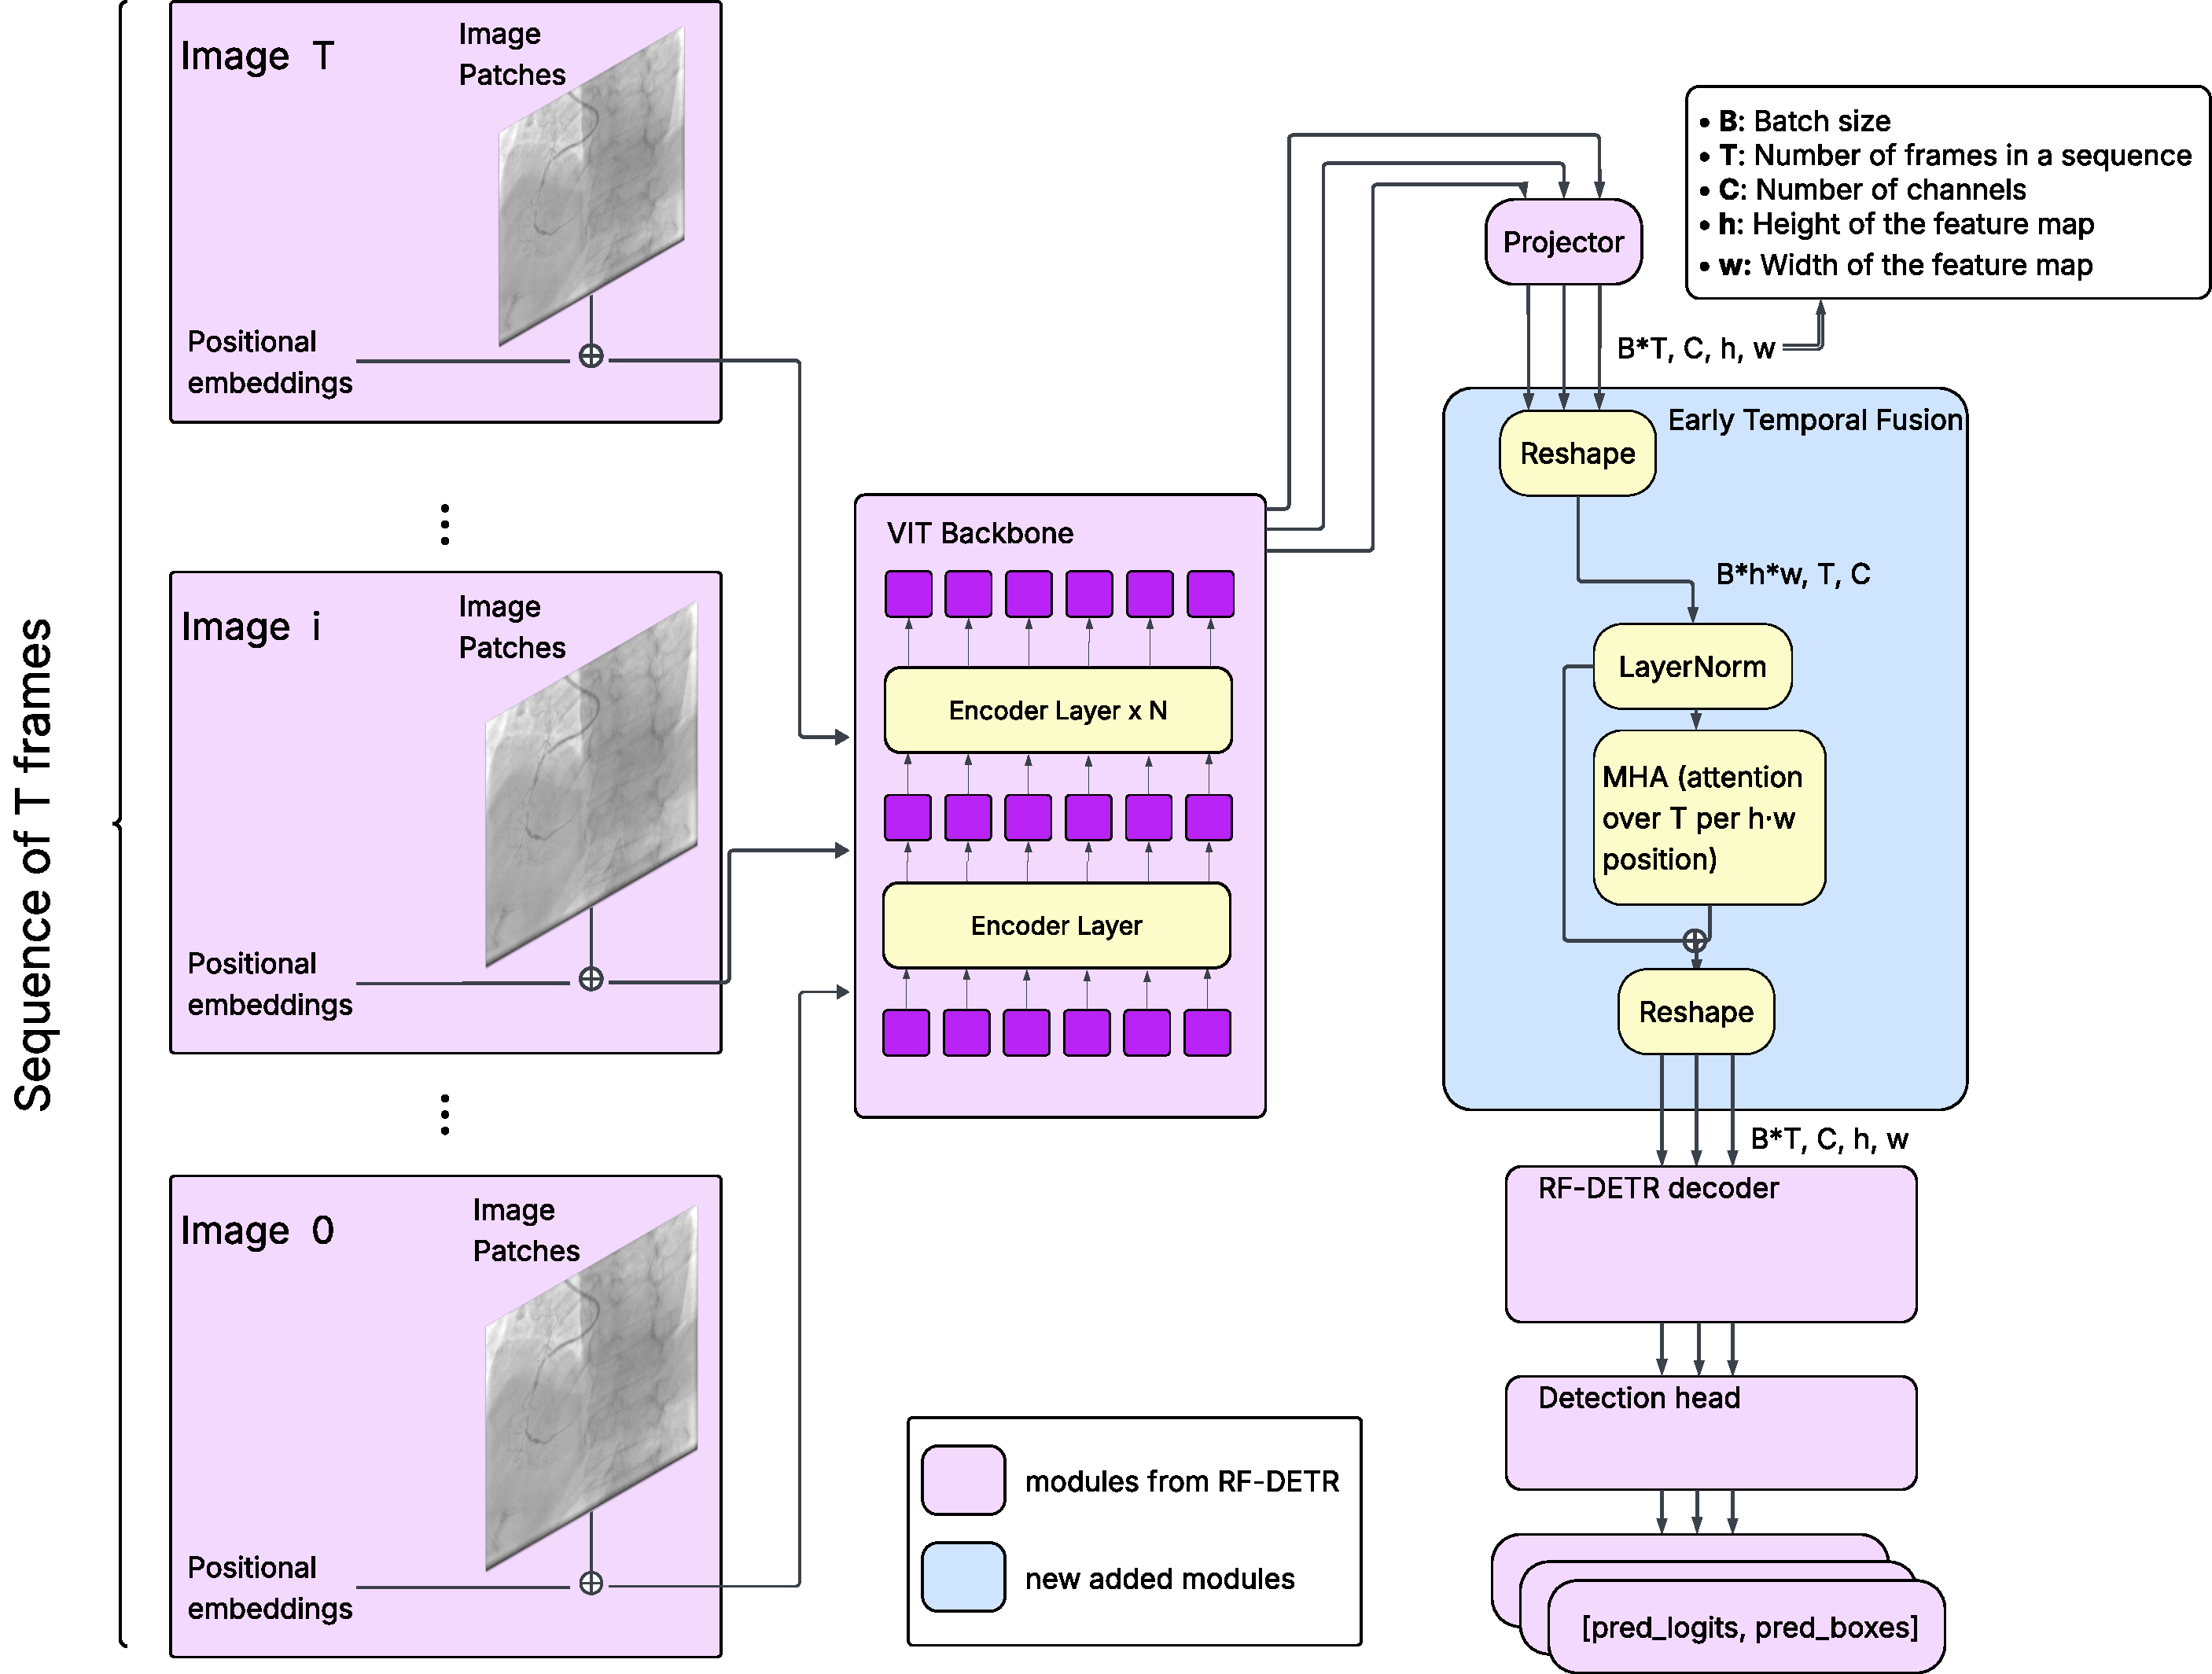
\includegraphics[width=0.92\textwidth]{TempoRF-DETR_final.pdf}
\caption{TempoRF-DETR architecture. MHA* in the Early Temporal Fusion module in the diagram stands for Multi-Head Attention.}
\label{fig:arch}
\end{figure*}

\subsection{TempoRF-DETR Architecture}
\label{sec:arch}

The architecture follows a simple design rule: the 2D RF-DETR pipeline is left untouched, and all cross-frame interaction is concentrated in a single inserted block. Every weight outside that block sees each frame exactly as the original 2D model did, so the full pretrained 2D RF-DETR checkpoint loads into the video model without modification. Concretely, a clip is a tensor of shape $(B, T, 3, H, W)$. We flatten the temporal axis into the batch axis so the unchanged RF-DETR DINOv2 backbone and projector see $(B\!\cdot\!T, 3, H, W)$ - that is, each of the $T$ frames is processed as an independent image - and they return multi-scale feature maps $\{F^{\ell}\}$ of shape $(B\!\cdot\!T, C, h_\ell, w_\ell)$. After the ETF block (below), the feature maps go through the standard RF-DETR transformer decoder and detection heads, still treating the flattened $(B\!\cdot\!T)$ axis as a batch. The model predicts every frame of the clip in one pass, returning $(B, T, Q, K)$ class logits and $(B, T, Q, 4)$ boxes.

\textbf{Early Temporal Fusion (ETF).} ETF is a single multi-head self-attention block that runs along the temporal axis of each backbone feature map. For one level $F^\ell$ of shape $(B\!\cdot\!T, C, h, w)$ we reshape to $(B\!\cdot\!h\!\cdot\!w,\, T,\, C)$ - one length-$T$ token sequence per spatial location - apply LayerNorm and Multi-Head Attention with $T$ queries/keys/values, and add the result back as a residual (Fig.~\ref{fig:arch}). Attention is purely position-wise: each spatial patch at location $(h, w)$ attends only to patches at the same $(h, w)$ position in the other $T-1$ frames, not across the whole feature map. The out-projection is zero-initialised, so ETF starts as an identity block and can be enabled safely from pretrained weights. ETF mixes information across all $T$ frames at every spatial location before the transformer decoder - this is what we call early fusion, in contrast to post-network or post-decoder tuning which only mix temporal information after the full per-frame detector has already run. Complexity is $\mathcal{O}(B\,h\,w\,C\,T^2)$ per level - quadratic in $T$ rather than in $h\,w\,T$ as a full spatio-temporal attention would be - so for small $T$ the cost is effectively linear in feature-map size.

\subsection{Image-to-Video Distillation}
\label{sec:distill}

\begin{figure*}[!htbp]
\centering
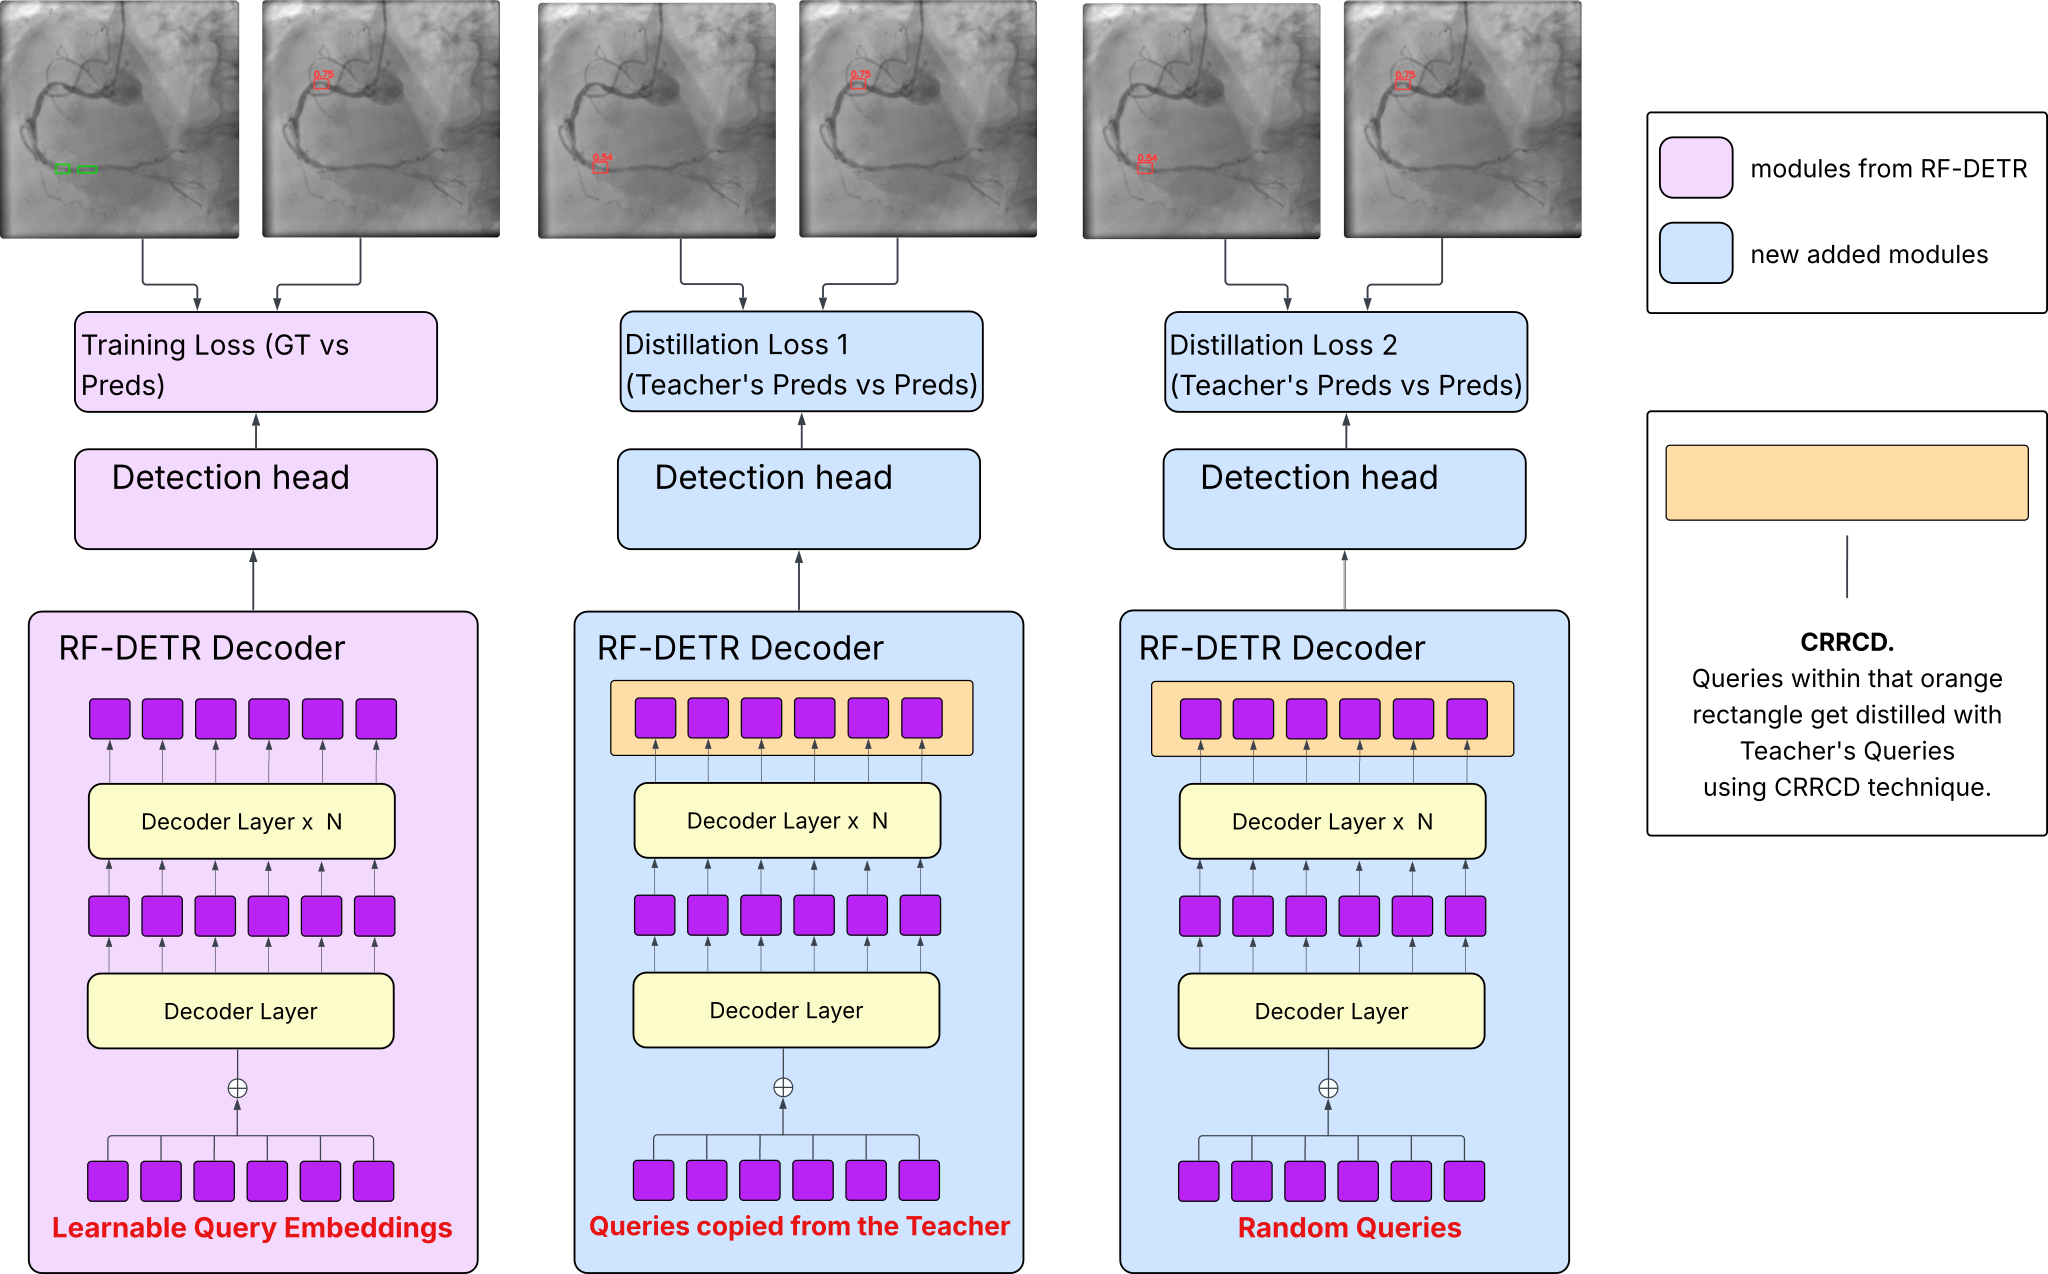
\includegraphics[width=0.92\textwidth]{Distillation_final_v2.pdf}
\caption{The three branches of image-to-video distillation.}
\label{fig:distill}
\end{figure*}

We choose distillation as the image-to-video bridging mechanism for two reasons. First, it is the cleanest way to combine our two supervision sources: a 2D teacher trained on the union of every available annotated frame (single-frame datasets and all decoded video frames) supervises the video student frame-by-frame, so the single-image data indirectly shapes the student even though the student never trains on it directly. Second, because we target an efficient model for clinical deployment, the video student is a smaller RF-DETR variant at lower input resolution; distilling from a slightly larger, same-architecture 2D teacher at higher resolution ($704$ vs.\ $512$) is a natural choice that adds spatial fidelity without additional cost, at the cost of a resolution gap that CRRCD (below) handles.

The frozen teacher's KD signal flows through three branches that share one backbone forward pass but differ in how they construct distillation points for the DETR family, following KD-DETR~\cite{wang2024kddetr} (Fig.~\ref{fig:distill}); we detail each below.

\textbf{Branch 1 (standard detection).} The student is queried with its own learnable queries and the standard RF-DETR set-prediction loss is applied per frame, $\mathcal{L}_{\text{det}} = \sum_{t} \mathcal{L}_{\text{set}}(s_t, y_t)$.

\textbf{Branch 2 (specific KD).} In DETR the teacher and student learn their object queries independently, so their $i$-th outputs need not describe the same object and cannot be compared directly. We remove this ambiguity by making the student reuse the teacher's queries: a forward pre-hook injects the exact queries the teacher feeds into its own decoder - object-query embeddings $\tilde{q}^{T}$ and reference points $\tilde{r}^{T}$ - into the student decoder in place of its learnable ones. With both decoders starting from the same queries, the student's $i$-th output describes the same candidate object as the teacher's and the two can be matched logit-for-logit:
\begin{equation}
\mathcal{L}_{\text{KD,sp}} = \sum_{i} w_i \!\left(\lambda_{\text{cls}}\, \ell^{\text{cls}}_i + \lambda_{\text{L1}}\, \ell^{\text{L1}}_i + \lambda_{\text{G}}\, \ell^{\text{G}}_i\right),
\label{eq:kd_specific}
\end{equation}
where $\ell^{\text{cls}}_i$ is a per-query KL term on class logits, $\ell^{\text{L1}}_i$ and $\ell^{\text{G}}_i$ are L1 and GIoU box losses between the student box $b_i^{s}$ and the teacher box $b_i^{t}$, and $w_i$ is KD-DETR's foreground-rebalance weight (the teacher's per-query foreground confidence).

\textbf{Branch 3 (general KD).} The teacher's queries from branch 2 are specialised toward confident foreground, so distilling through them alone teaches the student little about the rest of the image. We apply the same query-sharing trick with generic queries: $M_g$ fresh, uniformly-sampled queries (learned by neither model) are fed through both decoders, spreading supervision over the background and weakly-foreground locations the specific queries miss. The loss has the same form as~(\ref{eq:kd_specific}) with weight $\lambda_{\text{gen}}$ and a small floor weight $w^{g}_{\min}$ so background locations still pass a gradient.

\textbf{CRRCD on decoder hidden states.} Per-query logit distillation alone is brittle when teacher and student operate at different input resolutions: feature magnitudes shift in ways logits cannot compensate for. CRRCD~\cite{zhang2024crrcd} matches the relational structure of decoder hidden states $h^{s}, h^{t}$ between mini-batch samples rather than the states themselves. We sample foreground/background query slots per frame, project them through small MLPs $\phi^{s}, \phi^{t}$ into a shared relational space, and minimise
\begin{multline}
\mathcal{L}_{\text{CRRCD}} = -\!\!\sum_{(i,j)\in P}\!\! \log h(v^{t}_{i,j},\, v^{t,s}_{i,j}) \\
   -\, n\!\!\sum_{(i,j)\in N}\!\! \log\big[1 - h(v^{t}_{i,j},\, v^{t,s}_{i,j})\big],
\label{eq:crrcd}
\end{multline}
where $v^{t}_{i,j}$ is the teacher-space relation between samples $i,j$, $v^{t,s}_{i,j}$ the cross-space teacher-student relation, $h$ a temperature-scaled sigmoid critic that lower-bounds the mutual information between the two distributions~\cite{zhang2024crrcd}, and $n$ the number of negative pairs sampled per positive (set to $16$ in our experiments). As the relations are normalised in the projected space, absolute feature magnitudes need not match - only the geometry of foreground-background separation.

The total distillation loss is $\mathcal{L}_{\text{distill}} = \mathcal{L}_{\text{KD,sp}} + \lambda_{\text{gen}}\,\mathcal{L}_{\text{KD,gen}} + \lambda_{\text{CRRCD}}\,\mathcal{L}_{\text{CRRCD}}$, and the full training objective is $\mathcal{L} = \mathcal{L}_{\text{det}} + \lambda_{\text{distill}}\,\mathcal{L}_{\text{distill}}$, applied across all $T$ frames of the window. Geometric augmentations are replayed identically on student and teacher frames so that teacher targets remain spatially aligned with student predictions.

\section{Implementation}
\label{sec:impl}

\textbf{Models and inputs.} Both teacher and student keep the standard RF-DETR DINOv2 backbone, projector, transformer and detection heads; only ETF and the CRRCD relation MLPs are new. The teacher is RF-DETR Large at $704{\times}704$, pre-trained on the union of single-frame XCA data and decoded video frames (the same image-level data); the student is RF-DETR Small at $T{=}5$, $512{\times}512$ (matching XCA frame resolution; $T{>}5$ gave no gain in preliminary ablations), initialised from the corresponding 2D checkpoint trained on the same image-level union. The dataloader returns paired teacher ($704$) and student ($512$) frames with identical geometric augmentation; photometric augmentation is independent.

\textbf{Optimisation and losses.} We train for up to $50$ epochs on a single NVIDIA RTX~3060 (12\,GB) with AdamW, cosine schedule, $500$-iteration linear warm-up, batch size $4$, gradient accumulation $2$, weight decay $10^{-4}$, mixed-precision throughout. Learning rates are $10^{-4}$ for new modules (ETF, CRRCD MLPs), $3\!\times\!10^{-5}$ for pretrained transformer/heads, $10^{-5}$ for the backbone (kept frozen by default). Checkpoints are selected on the validation split by an EMA-smoothed score $(0.5\,\text{AP}_{0.3} + 0.3\,\text{AP}_{0.5} + 0.2\,\text{F1})$ with early stopping (patience $6$). Distillation weights: $\lambda_{\text{cls}}{=}2$, $\lambda_{\text{L1}}{=}5$, $\lambda_{\text{GIoU}}{=}2$, $\lambda_{\text{distill}}{=}1$, $\lambda_{\text{gen}}{=}0.5$ (specific floor $w_{\min}{=}0$, general floor $w^{g}_{\min}{=}0.1$, KL temperature $1$). CRRCD: $\lambda_{\text{CRRCD}}{=}2$, $16$ foreground / $32$ background queries per frame, $16$ negatives, temperature $0.1$, $256$-d relation space.

\textbf{Baselines and inference.} The parameter-efficient baselines freeze the same 2D RF-DETR backbone, transformer and heads (ETF, distillation, and CRRCD all disabled): \emph{Post-Network Tuning} adds a small temporal Transformer (1 layer, 8 heads) on top of the frozen decoder hidden states; \emph{Prompt Tuning} attaches $16$ learnable prompts propagated across frames via a small GRU. At inference we run overlapping $T{=}5$ windows (stride $1$) and keep the centre-frame prediction of each window; boundaries are edge-padded. Postprocessing is the standard sigmoid class threshold, no NMS. The model runs at $28.8$ FPS in fp16 on an RTX 3060 ($34.7$\,ms/frame, p95 $36.4$\,ms; $61.2$\,ms in fp32).

\section{Datasets and Evaluation}
\label{sec:datasets}

\textbf{Training and external validation datasets.} We use three public XCA datasets, exploiting the split between video and image data that motivates the distillation scheme. \textbf{RIPCID}~\cite{Danilov2021} - angiographic videos from $64$ patients ($214$ sequences, $8{,}323$ annotated frames) acquired on Philips Azurion~3 and Siemens Artis Zee systems - is our primary dataset, split patient-disjointly into train, validation, and test (test: $31$ sequences, $1{,}128$ centre frames). The split is constructed at the patient level so that no frame, sequence, or near-duplicate view from any patient appears in more than one split, ruling out the most common source of optimistic bias in medical-imaging benchmarks (data leakage through shared patients between train and test). \textbf{ARCADE}~\cite{popov2024arcade} - $1{,}500$ stenosis-annotated single-frame images from $1{,}500$ patients, acquired on Coroscop and Innova systems - is used as additional image-level supervision for the 2D teacher only. The teacher therefore trains on ARCADE $\cup$ decoded RIPCID-train; the video student trains only on RIPCID-train clips but is supervised per-frame by the teacher. \textbf{CADICA}~\cite{jimenezpartinen2024cadica} - videos from $28$ patients ($160$ sequences, $1{,}614$ centre frames, $2{,}284$ boxes) acquired on a Siemens Artis Zee system, with a different patient cohort and a different annotation team than RIPCID - is an entirely out-of-distribution (OOD) test set, never seen during training or model selection by any model.

\textbf{Metrics.} We report \emph{micro-pooled} (i.e.\ over all frames of all sequences in the split) AP at IoU thresholds $0.30$, $0.50$, as well as Precision (P), Recall (R), and F1 evaluated at the confidence that maximises micro F1 at IoU $0.30$. The choice of $0.30$ as the primary matching threshold is driven by our datasets, not by a clinical convention: we train and evaluate on three XCA resources whose ground-truth bounding-box sizes differ substantially (Fig.~\ref{fig:bbox_sizes}). RIPCID's median box covers only $0.28\%$ of the image (median side $\approx 5.3\%$ of the image side), roughly $3.2{\times}$ smaller in area than ARCADE ($0.91\%$, median side $\approx 9.5\%$) and $\sim 1.9{\times}$ smaller than CADICA ($0.52\%$, median side $\approx 7.3\%$) - a spread consistent with known inter-observer variability in XCA annotation~\cite{zir1976interobserver}. At RIPCID's scale a single-pixel localisation error already drops IoU below the standard $0.50$ threshold, so AP$_{50}$ and Precision/Recall at IoU $0.50$ over-penalise predictions whose centre is on the right vessel segment but whose extent is not pixel-perfect - and they do so unevenly across the three datasets because of the box-size gap. AP$_{30}$ gives a consistent operating point across all three. We therefore use micro-pooled AP$_{30}$ as the headline metric and report all Precision/Recall/F1 numbers at IoU $0.30$, with AP$_{50}$ and a full IoU sweep (Fig.~\ref{fig:ap_iou} in Appendix~\ref{app:appendix}) as additional context. All numbers in Section~\ref{sec:experiments} are reported on the held-out test split.

\textbf{Statistical testing.} To assess the significance of pairwise gaps we use the Wilcoxon signed-rank test on paired per-video AP$_{30}$ differences (one video = one patient cluster, the appropriate unit of independence). For each comparison, $H_0$: zero median per-video AP$_{30}$ difference between the two models; $H_1$: non-zero. All reported $p$-values are two-sided.

\begin{figure}[!t]
\centering
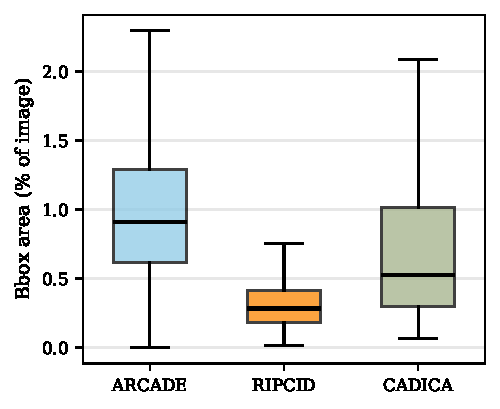
\includegraphics[width=0.72\columnwidth]{fig_bbox_sizes.pdf}
\caption{Ground-truth bbox area, as a fraction of image area, for the three XCA datasets. }
\label{fig:bbox_sizes}
\end{figure}

\section{Experiments and Results}
\label{sec:experiments}

All experiments are micro-pooled on the held-out test split.

\subsection{Ablation: Modules of TempoRF-DETR}
\label{sec:exp_ablation}

We progressively turned on each video-side component and reported micro-pooled AP$_{30}$ on RIPCID-test and CADICA (Table~\ref{tab:ablation_modules}). Rows 4-7 share the same TempoRF-DETR architecture: rows 4 vs.\ 5 isolate the 2D initialisation (RIPCID-only vs.\ ARCADE-augmented), while rows 6-7 add the KD and CRRCD distillation losses on top of row 5. Resolution, optimiser, and selection protocol were identical across rows.

\begin{table}[!t]
\centering
\caption{Module ablation, micro-pooled AP$_{30}$ on RIPCID-test (in-dist.) and CADICA (OOD). R = RIPCID, A = ARCADE; parentheticals list each 2D model's training data (row 3 is the teacher); \emph{init} picks which 2D checkpoint initialises the otherwise identical video student. Step p: Wilcoxon signed-rank two-sided p-value of the progressive video-block step on the OOD split, paired at the video level. $^{\dagger}$marginal CRRCD step is non-significant, but the combined KD + CRRCD step (row 5$\rightarrow$7) reaches $p=0.004$. In-distribution step p-values are all $\geq 0.075$.}
\label{tab:ablation_modules}
\footnotesize
\setlength{\tabcolsep}{4pt}
\begin{tabular}{clccc}
\hline
\textbf{\#} & \textbf{Model} & \textbf{R} & \textbf{CADICA} & \textbf{Step p (OOD)} \\
\hline
1 & 2D RF-DETR-S (R)              & 0.395 & 0.227 &  -  \\
2 & 2D RF-DETR-S (R+A)            & 0.445 & 0.390 &  -  \\
3 & 2D RF-DETR-L (R+A), teacher   & 0.460 & 0.401 &  -  \\
\hline
4 & Video ETF (R init)            & 0.471 & 0.241 &  -  \\
\hline
5 & Video ETF (R+A init)          & \textbf{0.582} & 0.370 & \textbf{$<$0.001} \\
6 & \quad + KD                    & 0.543 & 0.395 & \textbf{$<$0.001} \\
7 & \quad + KD + CRRCD (full)     & 0.581 & \textbf{0.416} & 0.13$^{\dagger}$ \\
\hline
\end{tabular}
\end{table}

The table shows three patterns worth pointing out. ARCADE supervision (rows 1$\rightarrow$2, and again via row-4 vs.\ row-5) is the dominant lever for the OOD column: without it the video student collapses on CADICA. ETF alone (row 2$\rightarrow$5) drives the in-distribution gain from temporal mixing but does not move OOD on its own. The distillation losses (rows 6-7) recover the in-distribution price of KD and add the rest of the OOD gain, bringing the full model above its 2D teacher on both splits; per-step significance is reported in the table's Step-p column. ETF-only (row 5) edges the full model in-distribution but within noise (ID step $p\geq 0.075$); we report the full model as headline for its OOD win.

\subsection{Comparison with Video Stenosis Detectors}
\label{sec:exp_video}

We reimplemented Stenosis-DetNet~\cite{PANG2021101900}, PS-STT~\cite{HAN2023106546}, and STQD-Det~\cite{STQD-Det} on the same RIPCID split and evaluation protocol so the comparison was not affected by data or metric differences. All three shared a ResNet-50 + FPN per-frame backbone with their respective temporal modules (SFF, proposal-shifted spatial-temporal Transformer, and STFS+quantum-diffusion box head), and were trained with $T=5$ frames at $512$ pixels for parity with TempoRF-DETR (Table~\ref{tab:video_methods}). Direct comparison with the originally reported F1$\,\approx\,0.88$-$0.92$ is not possible (private single-centre datasets, single-operating-point F1 at unstated IoU, no public code), but the published relative ordering STQD-Det $>$ Stenosis-DetNet $>$ PS-STT is preserved here.

\begin{table*}[!t]
\centering
\caption{Comparison with video stenosis detectors on RIPCID-test and CADICA (micro-pooled). All baselines are our reimplementations trained on RIPCID-train at $T{=}5$, $512$ resolution and identical evaluation pipeline. The \emph{p} column reports the Wilcoxon signed-rank two-sided p-value of the AP$_{30}$ gap to TempoRF-DETR, paired at the video level.}
\label{tab:video_methods}
\footnotesize
\begin{tabular}{lcccccc|cccccc}
\hline
& \multicolumn{6}{c|}{\textbf{RIPCID-test (in-distribution)}} & \multicolumn{6}{c}{\textbf{CADICA (out-of-distribution)}} \\
\textbf{Model} & AP$_{30}$ & AP$_{50}$ & P$_{30}$ & R$_{30}$ & F1$_{30}$ & \textbf{p} & AP$_{30}$ & AP$_{50}$ & P$_{30}$ & R$_{30}$ & F1$_{30}$ & \textbf{p} \\
\hline
Stenosis-DetNet~\cite{PANG2021101900} (ours, reimpl.)  & 0.328 & 0.130 & 0.454 & 0.371 & 0.408 & \textbf{0.012} & 0.089 & 0.015 & 0.211 & 0.199 & 0.205 & \textbf{$<$0.001} \\
PS-STT~\cite{HAN2023106546} (ours, reimpl.)            & 0.271 & 0.099 & 0.399 & 0.321 & 0.356 & \textbf{0.004} & 0.060 & 0.009 & 0.161 & 0.156 & 0.159 & \textbf{$<$0.001} \\
STQD-Det~\cite{STQD-Det} (ours, reimpl.)               & 0.377 & 0.169 & 0.569 & 0.497 & 0.531 & 0.32 \phantom{x} & 0.170 & 0.044 & 0.437 & 0.283 & 0.344 & \textbf{$<$0.001} \\
\textbf{TempoRF-DETR (ours)}                           & \textbf{0.581} & \textbf{0.247} & \textbf{0.710} & \textbf{0.515} & \textbf{0.597} &  -  & \textbf{0.416} & \textbf{0.111} & \textbf{0.609} & \textbf{0.383} & \textbf{0.470} &  -  \\
\hline
\end{tabular}
\end{table*}

TempoRF-DETR wins every column on both splits, and the gap widens out of distribution: the three baselines all stay below AP$_{30} = 0.18$ on CADICA. All three OOD gaps are significant at $p<0.001$ under the Wilcoxon signed-rank test; in-distribution, gaps to PS-STT and Stenosis-DetNet are significant ($p<0.05$), the gap to STQD-Det is not ($p=0.32$). Fig.~\ref{fig:methods_bar} summarises all six methods; qualitative detections are in Figs.~\ref{fig:qualitative_ripcid}-\ref{fig:qualitative_cadica}.

\begin{figure}[!t]
\centering
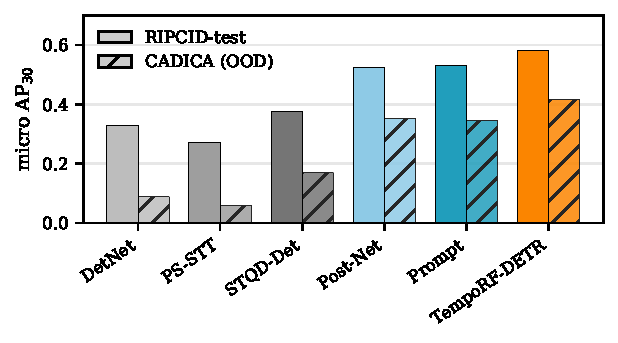
\includegraphics[width=0.95\columnwidth]{fig_methods_bar.pdf}
\caption{Micro-pooled AP$_{30}$ on RIPCID-test (solid) and CADICA (hatched, OOD) for all six methods. }
\label{fig:methods_bar}
\end{figure}

\subsection{Comparison with Image-to-Video Alternatives}
\label{sec:exp_pet}

We compared against two frozen-feature image-to-video alternatives from the survey of Li et al.~\cite{li2025imagetovideo}, trained on the same RIPCID split with the same frozen 2D RF-DETR backbone and the same $T{=}5$, $512$ student. Both modelled temporal information only \emph{after} the frozen per-frame features were computed, so they could not fix per-frame ambiguity at the feature level - precisely the gap our early-fusion and distillation design closes.

\begin{table*}[!t]
\centering
\caption{Image-to-video alternatives. Both baselines freeze the same 2D RF-DETR backbone, transformer, and heads, and train only the new temporal module; ETF, distillation, and CRRCD are disabled. The \emph{p} column reports the Wilcoxon signed-rank two-sided p-value of the AP$_{30}$ gap to TempoRF-DETR, paired at the video level.}
\label{tab:pet_methods}
\footnotesize
\begin{tabular}{lcccccc|cccccc}
\hline
& \multicolumn{6}{c|}{\textbf{RIPCID-test}} & \multicolumn{6}{c}{\textbf{CADICA}} \\
\textbf{Method} & AP$_{30}$ & AP$_{50}$ & P$_{30}$ & R$_{30}$ & F1$_{30}$ & \textbf{p} & AP$_{30}$ & AP$_{50}$ & P$_{30}$ & R$_{30}$ & F1$_{30}$ & \textbf{p} \\
\hline
Post-Network Tuning           & 0.525 & \textbf{0.278} & 0.568 & \textbf{0.589} & 0.578 & \textbf{0.028} & 0.353 & 0.112 & 0.506 & 0.373 & 0.430 & \textbf{0.046} \\
Prompt Tuning ($16$ prompts)  & 0.530 & 0.269 & 0.593 & 0.570 & 0.581 & \textbf{0.008} & 0.345 & \textbf{0.115} & 0.468 & \textbf{0.398} & 0.430 & \textbf{0.041} \\
\textbf{TempoRF-DETR (ours)}  & \textbf{0.581} & 0.247 & \textbf{0.710} & 0.515 & \textbf{0.597} &  -  & \textbf{0.416} & 0.111 & \textbf{0.609} & 0.383 & \textbf{0.470} &  -  \\
\hline
\end{tabular}
\end{table*}

TempoRF-DETR wins on AP$_{30}$ and F1$_{30}$ on both splits, trading slightly lower recall for noticeably higher precision; the OOD gap is the largest column-wise. The full AP-vs-IoU sweep is given in Fig.~\ref{fig:ap_iou} (Appendix~\ref{app:appendix}): on CADICA TempoRF-DETR stays on top at every IoU threshold, while in-distribution the order flips by a couple of points around the stricter AP$_{50}$. Under the Wilcoxon signed-rank test, all four AP$_{30}$ gaps to the PET alternatives are significant ($p<0.05$ both in-distribution and OOD).

\section{Discussion}

The video student exceeds its own static 2D teacher on both splits despite being smaller and lower-resolution - a direct demonstration that temporal information is additive to spatial information here; all headline gaps are tabulated in Tables~\ref{tab:video_methods}-\ref{tab:pet_methods}.

\textbf{What drives the gains, and how robust are they?} The most visible effect in the ablation (Table~\ref{tab:ablation_modules}) is that simply adding ARCADE to the teacher's training data is the largest single OOD jump in the table (rows 1$\rightarrow$2), before any video-side training, consistent with the cross-domain benefit of multi-source training~\cite{liu2020msnet, tetteh2021multidomain}; the same effect propagates to the video student, which collapses on CADICA when initialised from the RIPCID-only checkpoint (row 4) instead of the ARCADE-augmented one (row 2), making the ARCADE-augmented 2D checkpoint an essential prerequisite. ETF alone improves in-distribution but not OOD, because temporal mixing cannot inject cross-domain supervision on its own; the OOD gains come from the distillation losses. CRRCD's primary role within those losses is in-distribution stabilisation rather than direct metric gain: plain KD breaks the in-distribution feature geometry (row 5$\rightarrow$6) and CRRCD restores it to the ETF-baseline level (row 7), closing the $704\!\to\!512$ resolution gap between teacher and student that makes plain logit-level KD brittle. As a side-effect CRRCD also adds a small further OOD gain over the KD-only row, although this marginal step is at the edge of significance in isolation ($p=0.13$). Under the Wilcoxon signed-rank test, ARCADE pre-training, the OOD KD step, and the combined KD + CRRCD step over the ETF baseline are all significant on OOD ($p\leq 0.004$). Two honest caveats apply: the comparison to the video baselines in Table~\ref{tab:video_methods} is partly confounded by the stronger per-frame backbone (RF-DETR vs.\ ResNet-50 + FPN), and the in-distribution gap to STQD-Det collapses from $+0.204$ micro-pooled to $+0.047$ per-video macro and does not reach significance ($p=0.32$) - on most individual in-distribution videos the two methods sit at a comparable, SOTA-level operating point, and the substantive separation only appears on OOD ($p<0.001$).

\textbf{Generalisability of the approach.} The CADICA result is the most important practical outcome: a model trained on RIPCID $\cup$ ARCADE transfers without retraining to a previously unseen X-ray system and patient cohort at $0.416$ AP$_{30}$, more than double STQD-Det's $0.170$ and roughly $4.7{\times}$ Stenosis-DetNet's $0.089$. The cross-domain robustness comes from multi-source teacher training; image-to-video distillation just carries it through to the temporal student. In principle this freeze-and-distill recipe is not specific to stenosis and should carry over to other detection settings with the same data shape (abundant image data, scarce video data, deployment-time domain shift), though we do not test that here.

\textbf{Limitations and deployment.} TempoRF-DETR treats each $T$-frame window independently at inference, so long-range cardiac context spanning many beats is not exploited. Training requires running the teacher in parallel with the student, roughly doubling per-step compute. A fair cost-benefit observation: the OOD AP$_{30}$ gap between the 2D teacher (row 3 of Table~\ref{tab:ablation_modules}: $0.401$) and the full video model (row 7: $0.416$) is only $+0.015$, so multi-source 2D pre-training already does most of the cross-vendor work; the video pipeline's larger benefit ($+0.121$) is concentrated in-distribution. The case for the full pipeline therefore rests on the combination of in-distribution gain and OOD preservation, rather than OOD improvement in isolation. The CADICA evaluation is the only OOD test reported; broader cross-vendor evaluation with QCA endpoints is future work. On the deployment side the model runs at $28.8$\,FPS in fp16 on an RTX 3060 ($\approx 2$\,GB VRAM), well above the $15$\,FPS acquisition rate of a typical XCA scanner, and exports to ONNX without modification (ETF is a standard MHA*).

\section{Conclusion}

We presented TempoRF-DETR, a video extension of RF-DETR that adds a single early temporal-fusion (ETF) block before the detection transformer and is trained by distilling a frozen 2D teacher's per-frame knowledge into the video student via KD-DETR query alignment and cross-resolution relational contrastive distillation (CRRCD).

Returning to the three research questions: \textbf{(RQ1)} Yes - early temporal fusion makes the detector more accurate than both per-frame and prior video baselines. We are explicit about which split carries each significance claim: the gaps to the video baselines are statistically significant out of distribution for all three (Wilcoxon signed-rank) and in-distribution for the two weaker ones, while the in-distribution gap to the strongest baseline is large in aggregate but does not survive per-video aggregation, and the improvement over the per-frame teacher is reported as an effect size only. The evidence is therefore strongest out of distribution and supports a shift from single-frame to early-fused video modelling. \textbf{(RQ2)} Yes - image-to-video distillation lets the video student benefit from image-only data it never trains on directly. The effect is framed as a comparison between training conditions, not as a property of any single checkpoint: adding the single-frame source to the teacher, and then adding the distillation losses on top of the temporal baseline, each \emph{significantly improve} the student's out-of-distribution accuracy. Single-frame data the student never sees therefore measurably improves its predictions - not merely changes them - through the frozen teacher. \textbf{(RQ3)} Yes - the pipeline transfers to a previously unseen X-ray system and patient cohort without retraining, clearly outperforming the strongest reimplemented baseline. The ablation attributes this cross-vendor transfer to multi-source teacher pre-training rather than to the temporal architecture, which we read as a division of labour rather than a tension with RQ1: the ETF temporal block drives the in-distribution accuracy gain, while multi-source pre-training - carried into the student by distillation - drives the generalisation. The method's named temporal contribution thus earns its place on in-distribution quality, and we do not claim it as the source of cross-vendor transfer; two parameter-efficient frozen-feature alternatives fall short on AP$_{30}$ and F1$_{30}$ on both splits, supporting the early-fusion and distillation design over post-network adapters.

\begin{thebibliography}{00}
\bibitem{popov2022reviewmodernapproachescoronary} M. Popov, T. Aimyshev, E. Ismailov, A. Bulegenov, and S. Fazli, ``A Review of Modern Approaches for Coronary Angiography Imaging Analysis,'' arXiv preprint arXiv:2209.13997, 2022.

\bibitem{zir1976interobserver} L. M. Zir, S. W. Miller, R. E. Dinsmore, J. P. Gilbert, and J. W. Harthorne, ``Interobserver variability in coronary angiography,'' \textit{Circulation}, vol. 53, no. 4, pp. 627-632, 1976. doi: 10.1161/01.CIR.53.4.627

\bibitem{cardiovascular} H. Ren, F. Jing, Y. Fang, and W. Cheng, ``Artificial intelligence techniques for cardiovascular disease diagnosis via X-ray sensor-based coronary angiography: A bibliometric and systematic review,'' \textit{DIGITAL HEALTH}, vol. 12, p. 20552076261417142, 2026. doi: 10.1177/20552076261417142

\bibitem{MOON2021105819} J. H. Moon, D. Y. Lee, W. C. Cha, M. J. Chung, K.-S. Lee, B. H. Cho, and J. H. Choi, ``Automatic stenosis recognition from coronary angiography using convolutional neural networks,'' \textit{Computer Methods and Programs in Biomedicine}, vol. 198, p. 105819, 2021. doi: 10.1016/j.cmpb.2020.105819

\bibitem{Danilov2021} V. V. Danilov, K. Y. Klyshnikov, O. M. Gerget, et al., ``Real-time coronary artery stenosis detection based on modern neural networks,'' \textit{Scientific Reports}, vol. 11, no. 1, p. 7582, Apr. 2021. doi: 10.1038/s41598-021-87174-2

\bibitem{attentionstenosis} P. Van Stralen, D. L. Rodrigues, A. L. Oliveira, M. N. Menezes, and F. J. Pinto, ``Stenosis Detection in X-ray Coronary Angiography with Deep Neural Networks Leveraged by Attention Mechanisms,'' in \textit{Proc. 9th Int. Conf. Bioinformatics Research and Applications (ICBRA)}, 2023, pp. 123-128. doi: 10.1145/3569192.3569212

\bibitem{kupeli2025yolo} H. K\"upeli, I. Kuru, K. K. \c{C}evik, and A. Bozkurt, ``Angiography-Based Detection of Coronary Artery Stenosis Using YOLO Algorithm,'' \textit{Traitement du Signal}, vol. 42, no. 3, pp. 1525-1539, 2025. doi: 10.18280/ts.420325

\bibitem{aipoweredrealtime} K.-T. Tang, J.-Y. Shih, P. Hsu, C.-T. Liao, I.-M. Chiu, Z.-C. Chen, H.-L. Huang, L.-C. Yang, C. Liu, J. Wang, C.-H. Chang, J.-S. Huang, Y.-H. Hsu, M.-C. Tsai, N.-L. Chen, S.-H. Huang, K.-S. Chen, and W.-T. Chang, ``Artificial Intelligence Powered Real-Time Coronary Stenosis Recognition and Quantification in Angiography,'' \textit{Journal of Imaging Informatics in Medicine}, 2025. doi: 10.1007/s10278-025-01578-4

\bibitem{choudhary2026odysseiopensourceendtoendframework} A. Choudhary, X. Sun, T. Mahendiran, O. Senouf, D. Auberson, B. De Bruyne, S. Fournier, O. Muller, E. Abbé, P. Frossard, and D. Thanou, ``ODySSeI: An Open-Source End-to-End Framework for Automated Detection, Segmentation, and Severity Estimation of Lesions in Invasive Coronary Angiography Images,'' arXiv preprint arXiv:2603.20021, 2026.

\bibitem{fvcm} C. Cong, Y. Kato, H. D. De Vasconcellos, M. R. Ostovaneh, J. A. C. Lima, and B. Ambale-Venkatesh, ``Deep learning-based end-to-end automated stenosis classification and localization on catheter coronary angiography,'' \textit{Frontiers in Cardiovascular Medicine}, vol. 10, 2023. doi: 10.3389/fcvm.2023.944135

\bibitem{PANG2021101900} K. Pang, D. Ai, H. Fang, J. Fan, H. Song, and J. Yang, ``Stenosis-DetNet: Sequence consistency-based stenosis detection for X-ray coronary angiography,'' \textit{Computerized Medical Imaging and Graphics}, vol. 89, p. 101900, 2021. doi: 10.1016/j.compmedimag.2021.101900

\bibitem{HAN2023106546} T. Han, D. Ai, X. Li, J. Fan, H. Song, Y. Wang, and J. Yang, ``Coronary artery stenosis detection via proposal-shifted spatial-temporal transformer in X-ray angiography,'' \textit{Computers in Biology and Medicine}, vol. 153, p. 106546, 2023. doi: 10.1016/j.compbiomed.2023.106546

\bibitem{STQD-Det} X. Li, D. Ai, H. Song, J. Fan, T. Fu, D. Xiao, Y. Wang, and J. Yang, ``STQD-Det: Spatio-Temporal Quantum Diffusion Model for Real-Time Coronary Stenosis Detection in X-Ray Angiography,'' \textit{IEEE Transactions on Pattern Analysis and Machine Intelligence}, vol. 46, no. 12, pp. 9908-9920, 2024. doi: 10.1109/TPAMI.2024.3430839

\bibitem{li2025ltyolo} J. Li, X. Tang, and X. Wang, ``LT-YOLO: long-term temporal enhanced YOLO for stenosis detection on invasive coronary angiography,'' \textit{Frontiers in Molecular Biosciences}, vol. 12, p. 1558495, 2025. doi: 10.3389/fmolb.2025.1558495

\bibitem{huang2026vasomim} D.-X. Huang, C. Yu, X.-H. Zhou, T.-Y. Xiang, Q.-Y. Zhang, M.-J. Gui, R.-Z. Ma, C.-Y. Wang, N.-F. Xiao, F. Wang, and Z.-G. Hou, ``Vascular Anatomy-aware Self-supervised Pre-training for X-ray Angiogram Analysis,'' arXiv preprint arXiv:2602.11536, 2026.

\bibitem{liu2020msnet} Q. Liu, Q. Dou, L. Yu, and P. A. Heng, ``MS-Net: Multi-Site Network for Improving Prostate Segmentation With Heterogeneous MRI Data,'' \textit{IEEE Transactions on Medical Imaging}, vol. 39, no. 9, pp. 2713-2724, 2020. doi: 10.1109/TMI.2020.2974574

\bibitem{tetteh2021multidomain} E. Tetteh, J. Viviano, Y. Bengio, D. Krueger, and J. P. Cohen, ``Multi-Domain Balanced Sampling Improves Out-of-Distribution Generalization of Chest X-ray Pathology Prediction Models,'' in \textit{Medical Imaging Meets NeurIPS Workshop (Med-NeurIPS)}, 2021. arXiv:2112.13734.

\bibitem{popov2024arcade} M. Popov, A. Amanturdieva, N. Zhaksylyk, et al., ``Dataset for Automatic Region-based Coronary Artery Disease Diagnostics Using X-Ray Angiography Images,'' \textit{Scientific Data}, vol. 11, p. 20, 2024. doi: 10.1038/s41597-023-02871-z

\bibitem{li2025imagetovideo} J. Li, C. Tan, H. Chen, J. Ma, J.-F. Hu, J. Lai, and W.-S. Zheng, ``Image-to-Video Transfer Learning based on Image-Language Foundation Models: A Comprehensive Survey,'' arXiv preprint arXiv:2510.10671, 2025.

\bibitem{jimenezpartinen2024cadica} A. Jiménez-Partinen, M. A. Molina-Cabello, K. Thurnhofer-Hemsi, E. J. Palomo, J. Rodríguez-Capitán, A. I. Molina-Ramos, and M. Jiménez-Navarro, ``CADICA: a new dataset for coronary artery disease detection by using invasive coronary angiography,'' arXiv preprint arXiv:2402.00570, 2024.

\bibitem{girdhar2019distinit} R. Girdhar, D. Tran, L. Torresani, and D. Ramanan, ``DistInit: Learning Video Representations Without a Single Labeled Video,'' in \textit{Proc.\ IEEE/CVF International Conference on Computer Vision (ICCV)}, 2019, pp. 852-861. arXiv:1901.09244.

\bibitem{wang2024kddetr} Y. Wang, X. Li, S. Weng, G. Zhang, H. Yue, H. Feng, J. Han, and E. Ding, ``KD-DETR: Knowledge Distillation for Detection Transformer with Consistent Distillation Points Sampling,'' arXiv preprint arXiv:2211.08071, 2024.

\bibitem{zhang2024crrcd} K. Zhang, S. Ge, R. Shi, and D. Zeng, ``Low-Resolution Object Recognition with Cross-Resolution Relational Contrastive Distillation,'' \textit{IEEE Transactions on Circuits and Systems for Video Technology}, 2024. arXiv:2409.02555.

\end{thebibliography}

\clearpage
\onecolumn
\appendices
\section{Qualitative Detections and Full IoU Sweep}
\label{app:appendix}

\begin{figure}[H]
\centering
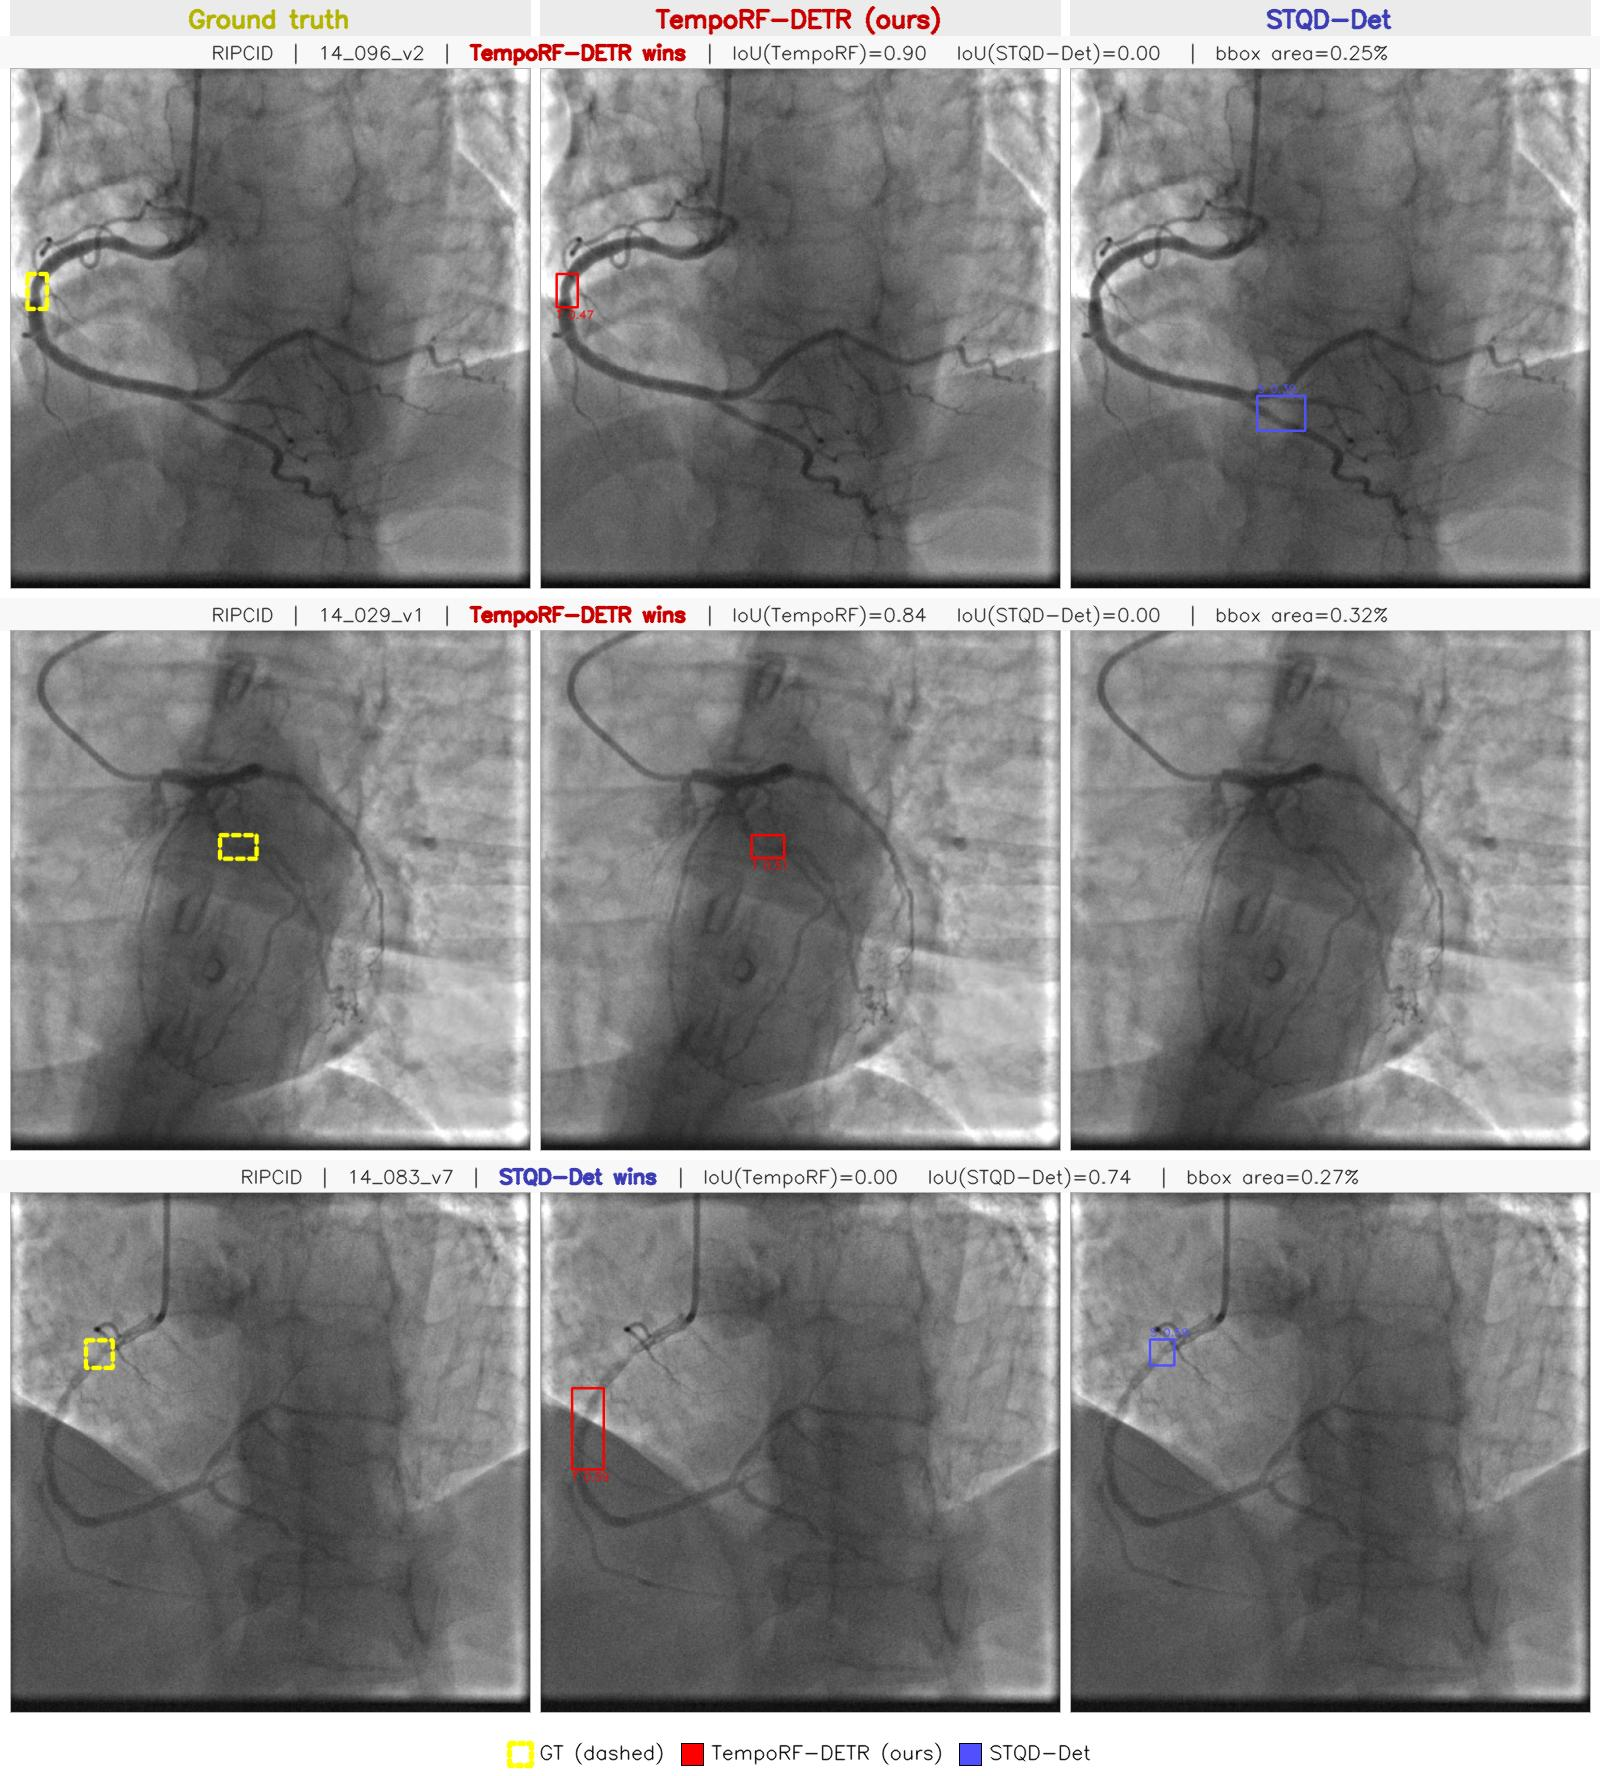
\includegraphics[width=\textwidth,keepaspectratio]{fig_qualitative_ripcid.pdf}
\caption{Qualitative examples on RIPCID-test (in-distribution). Three cases, one per row, with a title strip above each row giving dataset, sequence id, the winner under per-frame top-1 IoU, both IoU values, and the GT bbox area. The three columns of each row show the same full frame with, respectively, the ground-truth box only (yellow dashed), TempoRF-DETR's prediction only (red), and STQD-Det's prediction only (blue).}
\label{fig:qualitative_ripcid}
\end{figure}

\begin{figure}[H]
\centering
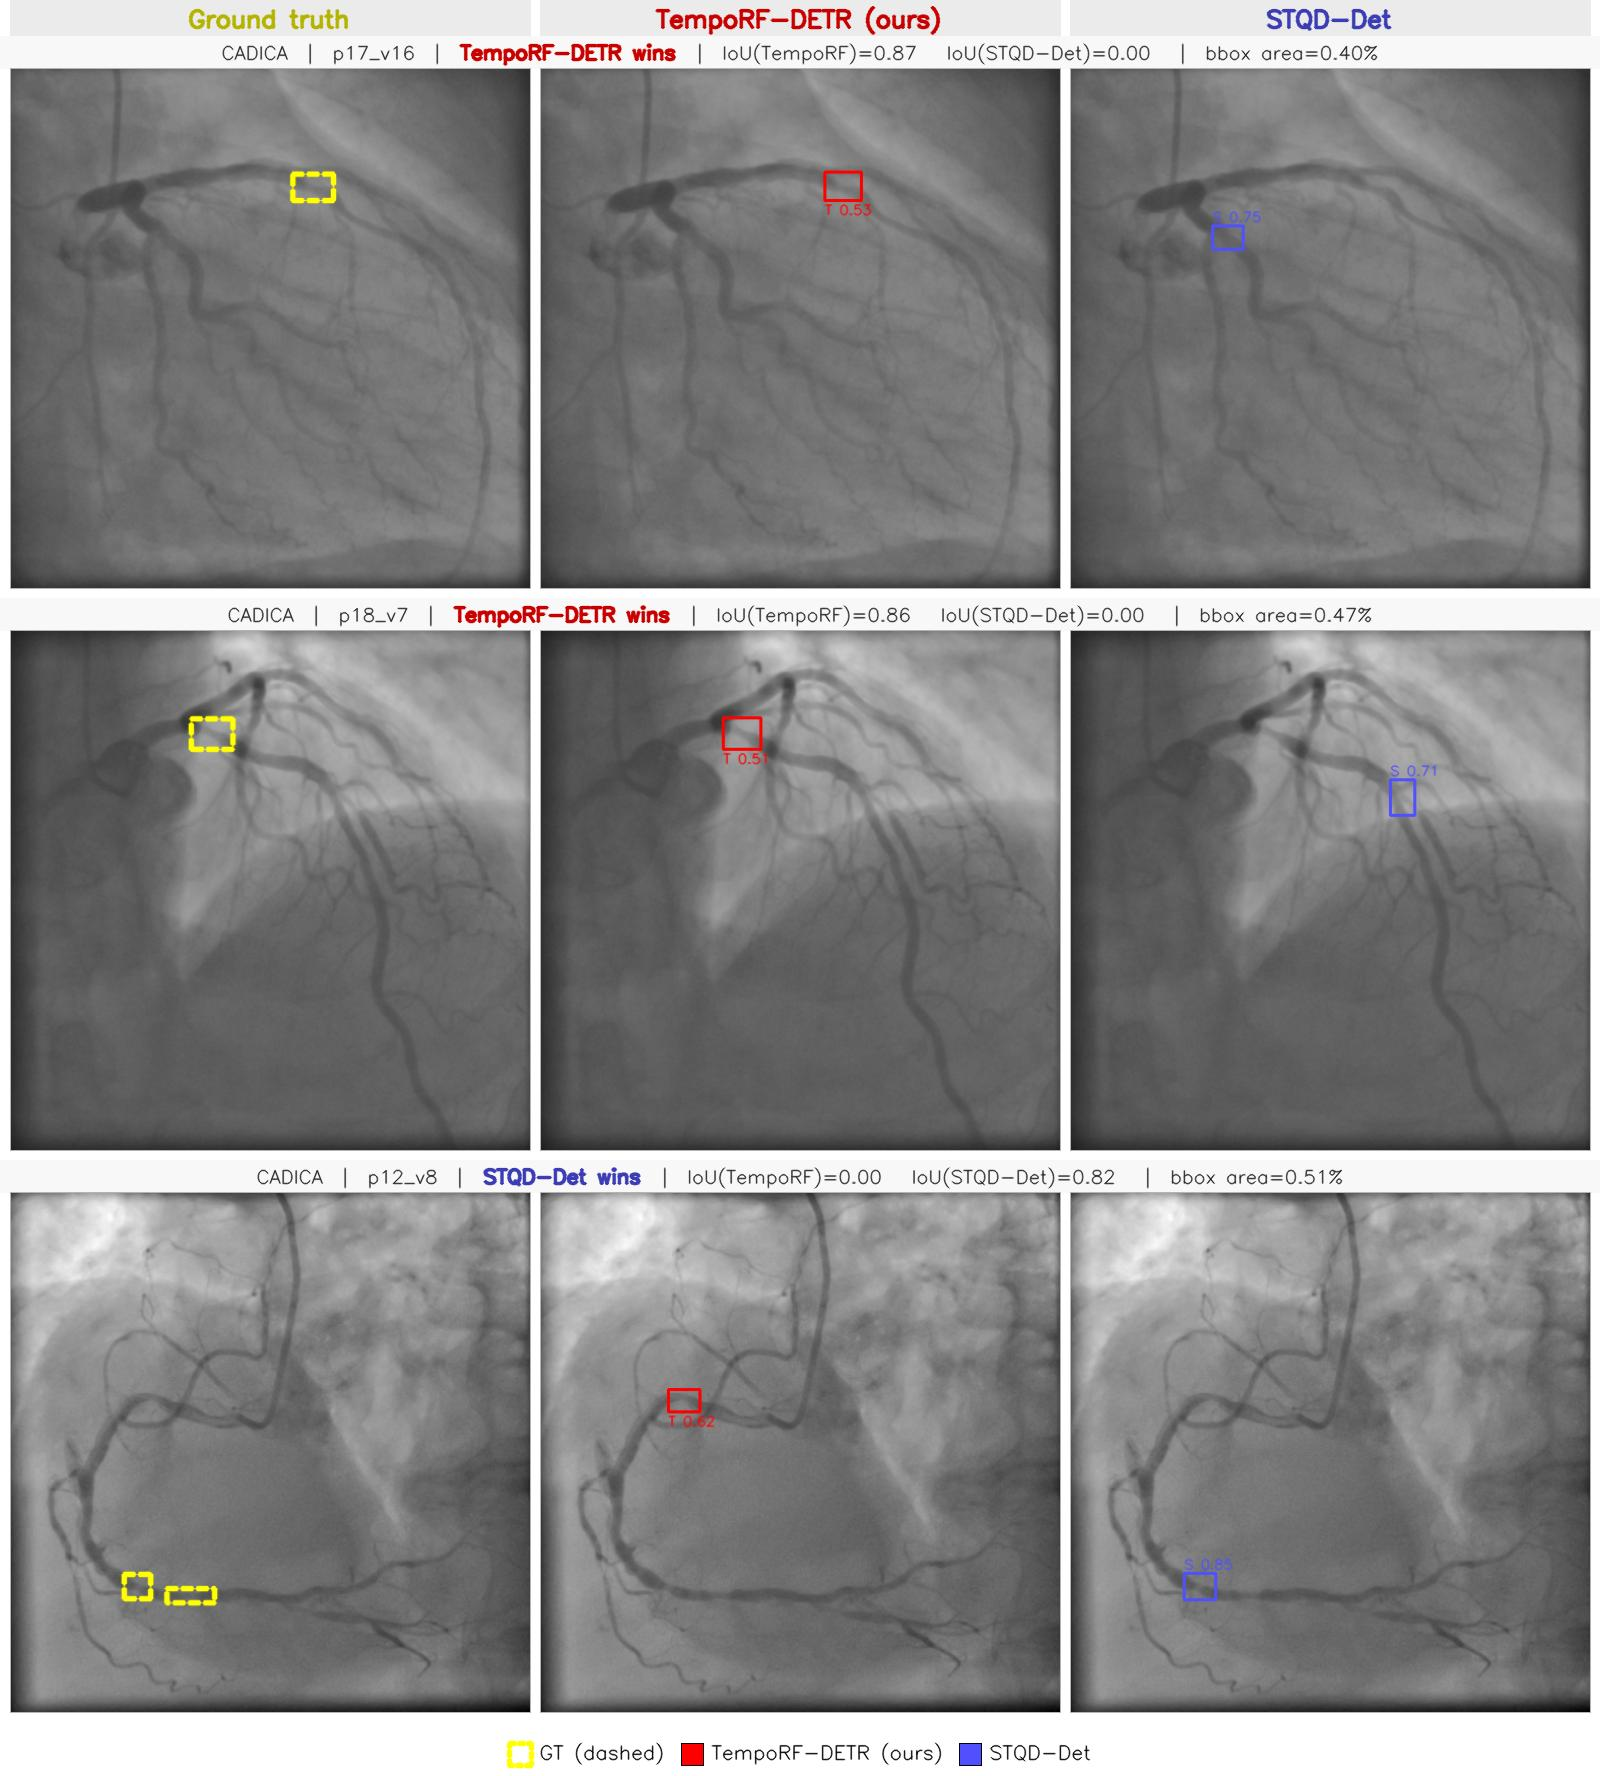
\includegraphics[width=\textwidth,keepaspectratio]{fig_qualitative_cadica.pdf}
\caption{Qualitative examples on CADICA (out-of-distribution). Same column layout as Fig.~\ref{fig:qualitative_ripcid}.}
\label{fig:qualitative_cadica}
\end{figure}

\begin{figure}[H]
\centering
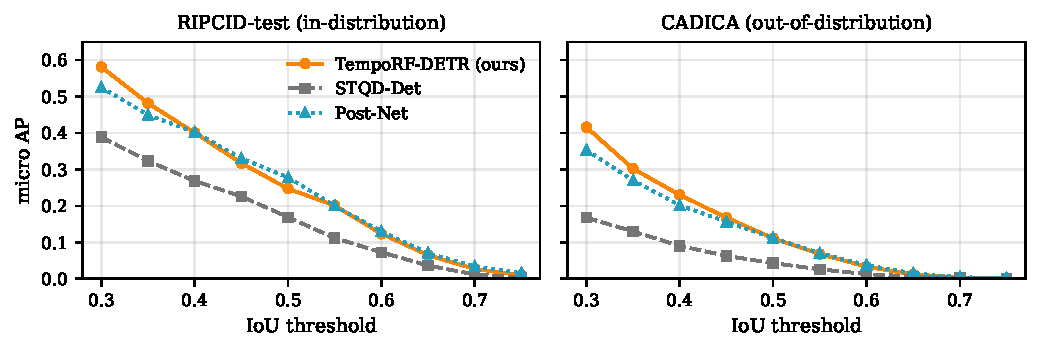
\includegraphics[width=0.95\textwidth]{fig_ap_iou.pdf}
\caption{Micro-pooled AP as a function of the IoU matching threshold for TempoRF-DETR (ours), STQD-Det (strongest reimplemented video baseline), and Post-Net (strongest parameter-efficient alternative).}
\label{fig:ap_iou}
\end{figure}

\end{document}
